\chapter{Testing Approach}

\section{General Test Procedure}

- Before starting a test case, the project is loaded to make sure that every test starts with the same program state
    - If this would not be done, it would be very hard to test programs that don't do proper initialization
    - Tests would depend on the state the previous test leaves the program in
    $\rightarrow$ Very inconsistent, therefore desirable to load the program before each test

- Then the test executes the program

\textit{- The test may press the green flag multiple times
- This allows to
    - test correct initialization of the program
    - test random values that are determined only once per program run
        - e.g. the program spawns a number of sprites in the beginning
        $\rightarrow$ only way to check if it's indeed random is to run the program multiple times
    }

\noindent- The test can then:
\begin{itemize}
    \item \textbf{Simulate Input}.
        - The test can simulate various user input.
        - It can simulate mouse movement, mouse button presses and keyboard button presses.
        - This is the only way the test can interact with the program.
        - The test should only interact with the program how a normal user would.

        - This work will explore automatic generation of input for Scratch programs
        - Input can be generated randomly
        - Static analysis can be used to detect the input events the program recognizes and to give the program inputs
        - A combination of both will be used for this work
    \item \textbf{Access Information}.
        - The test can select sprites by their name or by other condition (e.g. a sprite at a certain place).
        - It can also access the value of variables through the sprites the variables belong to.
        - Allows to check sprite positions, movement, animation, speech bubbles, etc.
        - Allows to check numbers that are displayed to the user
    \item \textbf{Control the program execution}.
        - The test can control how and for how long the program under test is run.
        - For example, the test can do some setup, then run the program until some sprite moves, then do some assertions.
    \item \textbf{Define constraints}.
        - The test can define constraints that must always hold true.
        - E.g. it can define that a sprite must never move left, or a sprite always moves in a certain direction when a key is pressed.
        - Needed because making assertions manually after every execution step is bothersome.
\end{itemize}

\noindent- The test can not:
\begin{itemize}
    \item \textbf{Directly manipulate properties of sprites or variables}.
        - The test should only interact with the program like a user would $\rightarrow$ realistic scenario
        - Directly manipulating sprites or variables could result in unexpected behaviour of the program
        $\rightarrow$ does not make sense for testing scratch programs
    \item \textbf{Execute single scripts or blocks directly}.
        - Block box approach does not allow to know anything about the code of the program (only names of sprites and variables)
        - Scratch programs are not made for modularity
            - Scripts are run in parallel
            - The given task could ask for isolated scripts that can be run on their own, but other languages are probably better suited for this

\end{itemize}

\section{Advantages and Disadvantages}

=== Shortcomings of this approach
- Scratch projects need to be well defined to be tested
    - Can take the creativity out of the process, but can also give the students a guide to follow, which helps them to not get stuck on one problem
    - Students can test their programs with the test suite beforehand on their own to verify their programs
    - Problem: might incentivize students to try to cheat the tests
        $\rightarrow$ Automated testing should only be used in conjunction with static analysis, manual analysis, or random secret tests
        (static analysis should easily show anomalies on the projects)
- Scratch programs can be pretty inconsistent
    - Some programs may only sometimes work and other times not
    $\rightarrow$ They may or may not pass the test

=== Advantages
- Allows the full range of Scratch functionality
    - ITCH only allows textual input and output, greatly limiting the possible functionality of tested programs
- Tests are easily understandable since they use the program like a normal user would
    - Students can test their programs with the test suite beforehand on their own to verify their programs
        $\rightarrow$ Students can easily receive feedback and will change their programs according to the tests
        $\rightarrow$ Incentivizes students to ask for help if they can't progress, because the test clearly shows that there is a problem

\section{Constraint-only Tests}%
\label{sec:constraint_only_tests}

- Normally, tests would deliberately simulate input on the program, then perform some assertions
- Constraints open up a new approach to testing Scratch programs by only defining constraints instead of doing normal assertions
- In the end of the test, it has to be checked if the desired situation for the constraint occurred during the program execution
    - E.g. a constraint that describes the movement speed of a sprite will always hold if the sprite does not move at all
    - $\rightarrow$ The constraint need to be filtered
- This makes it possible to separate the checking of properties from the execution of the program
    - Checks are only done through constraints, which run in the background
    $\rightarrow$ This is independent from the program execution
    $\rightarrow$ The program can be controlled by arbitrary input, as long as the desired situation for the constraint(s) comes about
        - Deliberately simulated input
        - Manual user input
        - Random input ($\rightarrow$ well-suited for random input, because the test is independent from the source of input)
          Similar approaches have been used in other testing applications, e.g. QuickCheck \ref{quickcheck}

- Normal tests vs. constraint-only tests
    - Normal tests can be more granular $\rightarrow$ better for grading
    - Normal tests allow to write very short tests for things that can be checked fast
        - More difficult if everything is tested in a single constraint-only test
        $\rightarrow$ Better for continuous development, because it's easier to quickly execute just one test
    - Constraint-only test require more processing, constraints have to be checked between every step
    - Constraints can't fully replace normal assertions: some properties are better checked with normal assertions (e.g. a property only has to hold for one point in time)

\begin{figure}[h]
    \centering
    \begin{subfigure}[b]{.45\textwidth}
        \centering
        \tikzset{>=latex,
                 box/.style={draw, text width=4.3cm, minimum height=0.7cm, text centered, rounded corners},
                 num/.style={draw, circle, inner sep=0.6mm, text centered},
                   h/.style={fill=blue!10}}

        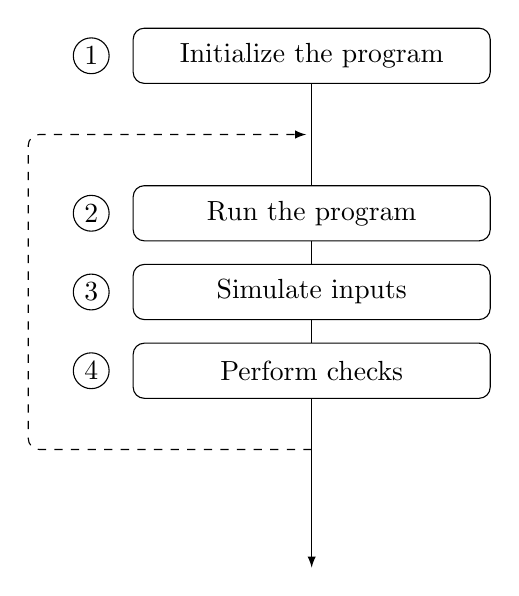
\begin{tikzpicture}
            \node[box] at ( 0.2,  5.0) (initialize) {Initialize the program};
            \node[box] at ( 0.2,  3.0) (run)        {Run the program};
            \node[box] at ( 0.2,  2.0) (inputs)     {Simulate inputs};
            \node[box] at ( 0.2,  1.0) (checks)     {Perform checks};

            \node[num] at (-2.6,  5.0) (one)   {1};
            \node[num] at (-2.6,  3.0) (two)   {2};
            \node[num] at (-2.6,  2.0) (three) {3};
            \node[num] at (-2.6,  1.0) (four)  {4};

            \draw[->]
                   (initialize)
                -- (run)
                -- (inputs)
                -- (checks)
                -- ( 0.2, -1.5);

            \draw[shorten >= 2pt, rounded corners, dashed, ->]
                   ( 0.2,  0.0)
                -- (-3.4,  0.0)
                -- (-3.4,  4.0)
                -- ( 0.2,  4.0);
        \end{tikzpicture}

        \caption{Normal Test Procedure}
        \label{fig:normal_test_procedure}
    \end{subfigure}
    \begin{subfigure}[b]{.45\textwidth}
        \centering
        \tikzset{>=latex,
                 box/.style={draw, text width=4.3cm, minimum height=0.7cm, text centered, rounded corners},
                 num/.style={draw, circle, inner sep=0.6mm, text centered},
                   h/.style={fill=blue!10}}

        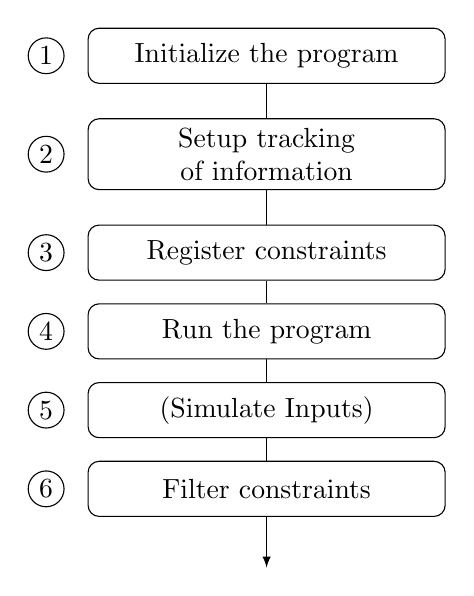
\begin{tikzpicture}
            \node[box] at ( 0.2,  5.5)  (initialize)  {Initialize the program};
            \node[box] at ( 0.2,  4.25) (tracking)    {Setup tracking of information};
            \node[box] at ( 0.2,  3.0)  (constraints) {Register constraints};
            \node[box] at ( 0.2,  2.0)  (run)         {Run the program};
            \node[box] at ( 0.2,  1.0)  (inputs)      {(Simulate Inputs)};
            \node[box] at ( 0.2,  0.0)  (filter)      {Filter constraints};

            \node[num] at (-2.6,  5.5)  (one)   {1};
            \node[num] at (-2.6,  4.25) (two)   {2};
            \node[num] at (-2.6,  3.0)  (three) {3};
            \node[num] at (-2.6,  2.0)  (four)  {4};
            \node[num] at (-2.6,  1.0)  (five)  {5};
            \node[num] at (-2.6,  0.0)  (six)   {6};

            \draw[->]
                   (initialize)
                -- (tracking)
                -- (constraints)
                -- (run)
                -- (inputs)
                -- (filter)
                -- ( 0.2, -1.0);
        \end{tikzpicture}

        \caption{Constraint-only Test Procedure}
        \label{fig:constraint_only_test_procedure}
    \end{subfigure}
    \caption{Comparison of the procedure of normal tests and constraint-only tests}
    \label{comparison_of_the_procedure_of_normal_tests_and_constraint_only_tests}
\end{figure}


